\documentclass[11pt]{article}
\usepackage[T1]{fontenc}
\usepackage[utf8]{inputenc}
\usepackage[a4paper,margin=25mm]{geometry}
\usepackage{amsmath,amssymb,amsthm,booktabs,tikz}
\usepackage[hidelinks]{hyperref}
\usepackage{microtype}
\setlength{\emergencystretch}{3em}
\makeatletter
\setlength{\@fptop}{0pt}
\setlength{\@fpsep}{14pt}
\setlength{\@fpbot}{0pt plus 1fil}
\makeatother
\definecolor{color0}{HTML}{F3EFE3}
\definecolor{color1}{HTML}{A8CEE8}
\definecolor{color2}{HTML}{F0B49B}
\definecolor{color3}{HTML}{B8D8B4}
\newtheorem{theorem}{Theorem}
\newtheorem{corollary}{Corollary}
\newtheorem{proposition}{Proposition}
\hypersetup{pdftitle={Explicit Three- and Four-Color Prismatic T-Tetrominoes},pdfauthor={Qiyuan Ma}}
\title{Explicit Three- and Four-Color Prismatic T-Tetrominoes}
\author{Qiyuan Ma\\
Shanghai Jiao Tong University\\
\href{mailto:mqyqwerty@sjtu.edu.cn}{\texttt{mqyqwerty@sjtu.edu.cn}}}
\date{24 October 2026}
\begin{document}
\maketitle

\begin{abstract}
We give explicit three- and four-color de Bruijn colorings of T-tetromino
ziggurats. The colorings have respectively 100 and 289 cells, and their 81
and 256 translated T-windows realize every ordered color pattern exactly
once. The known density theorem implies that both colorings are prismatic.
The established row-shift correspondence gives L-tetromino colorings with
the same parameters. We also exhibit 60 distinct labeled three-color
colorings. The complete color tables, machine-readable certificates, and
verification programs are supplied. Verification includes an independent
row-transfer computation of the known binary count of 168. These finite
results leave the five-color case and a construction for general color
number unsettled.
\end{abstract}

\section{Introduction}
Condon, Wang, and Yang introduced de Bruijn polyominoes: colored
polyominoes that contain exactly one translated copy of every coloring
of a fixed smaller polyomino \cite{CWY}. Their approach separates two
questions. First determine the smallest uncolored shape containing
enough copies of the smaller polyomino; then find a coloring that assigns
a different color pattern to each copy.

For the T tetromino, \cite[v2, Theorem 5.1]{CWY} determines the unique
dense shape when the required number of copies is a square. Its coloring
problem is left in \cite[v2, Remark 5.4]{CWY}, which gives the binary
example and a count of 168 binary colorings. Condon, Dugan, Goldman,
and Williams subsequently gave density formulas for further small
polyominoes \cite[Table 1]{CDGW}. In particular, their formula for the
T tetromino agrees with the area of the ziggurats considered here.

The purpose of this note is to supply explicit three- and four-color
T-tetromino certificates. The main result is Theorem~\ref{thm:main}; its
proof is a finite check of the complete tables printed below. The
corresponding L-tetromino result is a consequence of the known row-shift
bijection. A small explicit family gives a three-color counting lower
bound. The accompanying programs separate certificate verification,
restricted counting, and the search models used to obtain the examples.

\section{Notation and density}
A cell is identified with its integer lattice coordinate. A polyomino
is a finite, edge-connected set of cells. All small shapes have fixed
orientation, and only their translates are counted. Set
\[
 T=\{(0,1),(-1,0),(0,0),(1,0)\},\qquad
 Z_m=\{(j-r,-r):0\le r\le m,\ 0\le j\le2r\}.
\]
Thus $Z_m$ is a ziggurat of height $m+1$, with row lengths
$1,3,\ldots,2m+1$. An $n$-coloring assigns each cell a label from
$\{0,1,\ldots,n-1\}$. The ordered pattern of a translated $T$ is read
as (top, left, middle, right).

Following \cite[v2]{CWY}, a $(T,n)$-de Bruijn coloring contains each of
the $n^4$ ordered patterns exactly once. A $(T,N)$-dense polyomino has
minimum area among polyominoes containing at least $N$ translates of $T$.
A $(T,n)$-de Bruijn coloring on a $(T,n^4)$-dense shape is called
\emph{prismatic}. This definition of prismatic is the one used in the
revised version of \cite{CWY}.

Write $a_r(j)$ for the color of the cell $(j-r,-r)$. Every T-window of
$Z_m$ is indexed uniquely by
\begin{equation}\label{eq:window}
 \bigl(a_{r-1}(j),a_r(j),a_r(j+1),a_r(j+2)\bigr),\qquad
 1\le r\le m,\quad0\le j\le2r-2.
\end{equation}
Indeed its lower middle cell must have both horizontal neighbors and
a cell immediately above it, and these conditions give precisely the
stated index ranges.

\begin{proposition}\label{prop:geometry}
The ziggurat $Z_{n^2}$ has $(n^2+1)^2$ cells and exactly $n^4$ T-windows.
\end{proposition}
\begin{proof}
Its number of cells is
$\sum_{r=0}^{n^2}(2r+1)=(n^2+1)^2$. Between rows $r-1$ and $r$,
\eqref{eq:window} gives $2r-1$ windows, so their total is
$\sum_{r=1}^{n^2}(2r-1)=(n^2)^2=n^4$.
\end{proof}

Theorem 5.1 of \cite[v2]{CWY} states that $Z_N$ is the unique
$(T,N^2)$-dense shape, up to translation. Applying it with $N=n^2$
shows that $Z_{n^2}$ is $(T,n^4)$-dense. Equivalently,
\cite[Table 1]{CDGW} gives
\[
 a_{T,N}=\left\lceil N+\sqrt{4N}+1\right\rceil,
 \qquad a_{T,n^4}=(n^2+1)^2.
\]
Consequently, a de Bruijn coloring of $Z_{n^2}$ is prismatic.

\section{Explicit colorings}
\begin{theorem}\label{thm:main}
For each $n\in\{3,4\}$, the ziggurat $Z_{n^2}$ admits a
$(T,n)$-prismatic coloring. Tables~\ref{tab:n3} and~\ref{tab:n4}
give such colorings.
\end{theorem}
\begin{proof}[Verification of the certificates]
Read each row of the appropriate table from left to right. All row
lengths and color labels have the required ranges. For a window
$(t,l,c,u)$, form its integer code
\[
 E_n(t,l,c,u)=n^3t+n^2l+nc+u.
\]
Evaluating \eqref{eq:window} on Table~\ref{tab:n3} gives each integer
from 0 to 80 exactly once; on Table~\ref{tab:n4} it gives each integer
from 0 to 255 exactly once. Thus both tables are de Bruijn colorings.
The density result above proves that they are prismatic.

These finite checks can be verified directly from the tables or by the
supplied program \path{verify.py}. The files \path{n3_patterns.csv} and
\path{n4_patterns.csv} give the unique index $(r,j)$ for each pattern
in increasing code order. The program also regenerates all translated
windows from planar coordinates, independently of the row-indexed
enumeration.
\end{proof}

\begin{table}[ht]
\centering
\small
\begin{tabular}{r l}\toprule
Row $r$ & Colors, left to right \\\midrule
0 & \texttt{0} \\
1 & \texttt{000} \\
2 & \texttt{00100} \\
3 & \texttt{0020110} \\
4 & \texttt{012021022} \\
5 & \texttt{10110211112} \\
6 & \texttt{0121222022001} \\
7 & \texttt{122101020222001} \\
8 & \texttt{22211121210122112} \\
9 & \texttt{1201100021201000200} \\
\bottomrule\end{tabular}
\caption{A complete three-color certificate on $Z_9$.}\label{tab:n3}
\end{table}
\begin{figure}[ht]
\centering
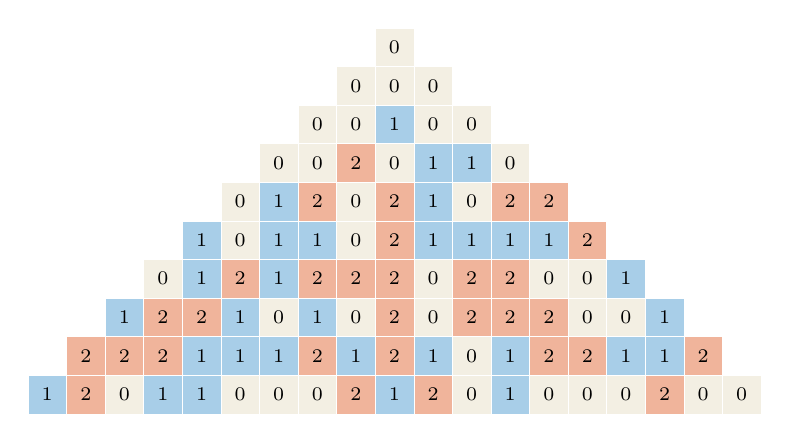
\begin{tikzpicture}[x=0.49cm,y=0.49cm]
\filldraw[fill=color0,draw=white,line width=0.2pt] (0,0) rectangle ++(1,1);
\node[font=\scriptsize] at (0.5,0.5) {0};
\filldraw[fill=color0,draw=white,line width=0.2pt] (-1,-1) rectangle ++(1,1);
\node[font=\scriptsize] at (-0.5,-0.5) {0};
\filldraw[fill=color0,draw=white,line width=0.2pt] (0,-1) rectangle ++(1,1);
\node[font=\scriptsize] at (0.5,-0.5) {0};
\filldraw[fill=color0,draw=white,line width=0.2pt] (1,-1) rectangle ++(1,1);
\node[font=\scriptsize] at (1.5,-0.5) {0};
\filldraw[fill=color0,draw=white,line width=0.2pt] (-2,-2) rectangle ++(1,1);
\node[font=\scriptsize] at (-1.5,-1.5) {0};
\filldraw[fill=color0,draw=white,line width=0.2pt] (-1,-2) rectangle ++(1,1);
\node[font=\scriptsize] at (-0.5,-1.5) {0};
\filldraw[fill=color1,draw=white,line width=0.2pt] (0,-2) rectangle ++(1,1);
\node[font=\scriptsize] at (0.5,-1.5) {1};
\filldraw[fill=color0,draw=white,line width=0.2pt] (1,-2) rectangle ++(1,1);
\node[font=\scriptsize] at (1.5,-1.5) {0};
\filldraw[fill=color0,draw=white,line width=0.2pt] (2,-2) rectangle ++(1,1);
\node[font=\scriptsize] at (2.5,-1.5) {0};
\filldraw[fill=color0,draw=white,line width=0.2pt] (-3,-3) rectangle ++(1,1);
\node[font=\scriptsize] at (-2.5,-2.5) {0};
\filldraw[fill=color0,draw=white,line width=0.2pt] (-2,-3) rectangle ++(1,1);
\node[font=\scriptsize] at (-1.5,-2.5) {0};
\filldraw[fill=color2,draw=white,line width=0.2pt] (-1,-3) rectangle ++(1,1);
\node[font=\scriptsize] at (-0.5,-2.5) {2};
\filldraw[fill=color0,draw=white,line width=0.2pt] (0,-3) rectangle ++(1,1);
\node[font=\scriptsize] at (0.5,-2.5) {0};
\filldraw[fill=color1,draw=white,line width=0.2pt] (1,-3) rectangle ++(1,1);
\node[font=\scriptsize] at (1.5,-2.5) {1};
\filldraw[fill=color1,draw=white,line width=0.2pt] (2,-3) rectangle ++(1,1);
\node[font=\scriptsize] at (2.5,-2.5) {1};
\filldraw[fill=color0,draw=white,line width=0.2pt] (3,-3) rectangle ++(1,1);
\node[font=\scriptsize] at (3.5,-2.5) {0};
\filldraw[fill=color0,draw=white,line width=0.2pt] (-4,-4) rectangle ++(1,1);
\node[font=\scriptsize] at (-3.5,-3.5) {0};
\filldraw[fill=color1,draw=white,line width=0.2pt] (-3,-4) rectangle ++(1,1);
\node[font=\scriptsize] at (-2.5,-3.5) {1};
\filldraw[fill=color2,draw=white,line width=0.2pt] (-2,-4) rectangle ++(1,1);
\node[font=\scriptsize] at (-1.5,-3.5) {2};
\filldraw[fill=color0,draw=white,line width=0.2pt] (-1,-4) rectangle ++(1,1);
\node[font=\scriptsize] at (-0.5,-3.5) {0};
\filldraw[fill=color2,draw=white,line width=0.2pt] (0,-4) rectangle ++(1,1);
\node[font=\scriptsize] at (0.5,-3.5) {2};
\filldraw[fill=color1,draw=white,line width=0.2pt] (1,-4) rectangle ++(1,1);
\node[font=\scriptsize] at (1.5,-3.5) {1};
\filldraw[fill=color0,draw=white,line width=0.2pt] (2,-4) rectangle ++(1,1);
\node[font=\scriptsize] at (2.5,-3.5) {0};
\filldraw[fill=color2,draw=white,line width=0.2pt] (3,-4) rectangle ++(1,1);
\node[font=\scriptsize] at (3.5,-3.5) {2};
\filldraw[fill=color2,draw=white,line width=0.2pt] (4,-4) rectangle ++(1,1);
\node[font=\scriptsize] at (4.5,-3.5) {2};
\filldraw[fill=color1,draw=white,line width=0.2pt] (-5,-5) rectangle ++(1,1);
\node[font=\scriptsize] at (-4.5,-4.5) {1};
\filldraw[fill=color0,draw=white,line width=0.2pt] (-4,-5) rectangle ++(1,1);
\node[font=\scriptsize] at (-3.5,-4.5) {0};
\filldraw[fill=color1,draw=white,line width=0.2pt] (-3,-5) rectangle ++(1,1);
\node[font=\scriptsize] at (-2.5,-4.5) {1};
\filldraw[fill=color1,draw=white,line width=0.2pt] (-2,-5) rectangle ++(1,1);
\node[font=\scriptsize] at (-1.5,-4.5) {1};
\filldraw[fill=color0,draw=white,line width=0.2pt] (-1,-5) rectangle ++(1,1);
\node[font=\scriptsize] at (-0.5,-4.5) {0};
\filldraw[fill=color2,draw=white,line width=0.2pt] (0,-5) rectangle ++(1,1);
\node[font=\scriptsize] at (0.5,-4.5) {2};
\filldraw[fill=color1,draw=white,line width=0.2pt] (1,-5) rectangle ++(1,1);
\node[font=\scriptsize] at (1.5,-4.5) {1};
\filldraw[fill=color1,draw=white,line width=0.2pt] (2,-5) rectangle ++(1,1);
\node[font=\scriptsize] at (2.5,-4.5) {1};
\filldraw[fill=color1,draw=white,line width=0.2pt] (3,-5) rectangle ++(1,1);
\node[font=\scriptsize] at (3.5,-4.5) {1};
\filldraw[fill=color1,draw=white,line width=0.2pt] (4,-5) rectangle ++(1,1);
\node[font=\scriptsize] at (4.5,-4.5) {1};
\filldraw[fill=color2,draw=white,line width=0.2pt] (5,-5) rectangle ++(1,1);
\node[font=\scriptsize] at (5.5,-4.5) {2};
\filldraw[fill=color0,draw=white,line width=0.2pt] (-6,-6) rectangle ++(1,1);
\node[font=\scriptsize] at (-5.5,-5.5) {0};
\filldraw[fill=color1,draw=white,line width=0.2pt] (-5,-6) rectangle ++(1,1);
\node[font=\scriptsize] at (-4.5,-5.5) {1};
\filldraw[fill=color2,draw=white,line width=0.2pt] (-4,-6) rectangle ++(1,1);
\node[font=\scriptsize] at (-3.5,-5.5) {2};
\filldraw[fill=color1,draw=white,line width=0.2pt] (-3,-6) rectangle ++(1,1);
\node[font=\scriptsize] at (-2.5,-5.5) {1};
\filldraw[fill=color2,draw=white,line width=0.2pt] (-2,-6) rectangle ++(1,1);
\node[font=\scriptsize] at (-1.5,-5.5) {2};
\filldraw[fill=color2,draw=white,line width=0.2pt] (-1,-6) rectangle ++(1,1);
\node[font=\scriptsize] at (-0.5,-5.5) {2};
\filldraw[fill=color2,draw=white,line width=0.2pt] (0,-6) rectangle ++(1,1);
\node[font=\scriptsize] at (0.5,-5.5) {2};
\filldraw[fill=color0,draw=white,line width=0.2pt] (1,-6) rectangle ++(1,1);
\node[font=\scriptsize] at (1.5,-5.5) {0};
\filldraw[fill=color2,draw=white,line width=0.2pt] (2,-6) rectangle ++(1,1);
\node[font=\scriptsize] at (2.5,-5.5) {2};
\filldraw[fill=color2,draw=white,line width=0.2pt] (3,-6) rectangle ++(1,1);
\node[font=\scriptsize] at (3.5,-5.5) {2};
\filldraw[fill=color0,draw=white,line width=0.2pt] (4,-6) rectangle ++(1,1);
\node[font=\scriptsize] at (4.5,-5.5) {0};
\filldraw[fill=color0,draw=white,line width=0.2pt] (5,-6) rectangle ++(1,1);
\node[font=\scriptsize] at (5.5,-5.5) {0};
\filldraw[fill=color1,draw=white,line width=0.2pt] (6,-6) rectangle ++(1,1);
\node[font=\scriptsize] at (6.5,-5.5) {1};
\filldraw[fill=color1,draw=white,line width=0.2pt] (-7,-7) rectangle ++(1,1);
\node[font=\scriptsize] at (-6.5,-6.5) {1};
\filldraw[fill=color2,draw=white,line width=0.2pt] (-6,-7) rectangle ++(1,1);
\node[font=\scriptsize] at (-5.5,-6.5) {2};
\filldraw[fill=color2,draw=white,line width=0.2pt] (-5,-7) rectangle ++(1,1);
\node[font=\scriptsize] at (-4.5,-6.5) {2};
\filldraw[fill=color1,draw=white,line width=0.2pt] (-4,-7) rectangle ++(1,1);
\node[font=\scriptsize] at (-3.5,-6.5) {1};
\filldraw[fill=color0,draw=white,line width=0.2pt] (-3,-7) rectangle ++(1,1);
\node[font=\scriptsize] at (-2.5,-6.5) {0};
\filldraw[fill=color1,draw=white,line width=0.2pt] (-2,-7) rectangle ++(1,1);
\node[font=\scriptsize] at (-1.5,-6.5) {1};
\filldraw[fill=color0,draw=white,line width=0.2pt] (-1,-7) rectangle ++(1,1);
\node[font=\scriptsize] at (-0.5,-6.5) {0};
\filldraw[fill=color2,draw=white,line width=0.2pt] (0,-7) rectangle ++(1,1);
\node[font=\scriptsize] at (0.5,-6.5) {2};
\filldraw[fill=color0,draw=white,line width=0.2pt] (1,-7) rectangle ++(1,1);
\node[font=\scriptsize] at (1.5,-6.5) {0};
\filldraw[fill=color2,draw=white,line width=0.2pt] (2,-7) rectangle ++(1,1);
\node[font=\scriptsize] at (2.5,-6.5) {2};
\filldraw[fill=color2,draw=white,line width=0.2pt] (3,-7) rectangle ++(1,1);
\node[font=\scriptsize] at (3.5,-6.5) {2};
\filldraw[fill=color2,draw=white,line width=0.2pt] (4,-7) rectangle ++(1,1);
\node[font=\scriptsize] at (4.5,-6.5) {2};
\filldraw[fill=color0,draw=white,line width=0.2pt] (5,-7) rectangle ++(1,1);
\node[font=\scriptsize] at (5.5,-6.5) {0};
\filldraw[fill=color0,draw=white,line width=0.2pt] (6,-7) rectangle ++(1,1);
\node[font=\scriptsize] at (6.5,-6.5) {0};
\filldraw[fill=color1,draw=white,line width=0.2pt] (7,-7) rectangle ++(1,1);
\node[font=\scriptsize] at (7.5,-6.5) {1};
\filldraw[fill=color2,draw=white,line width=0.2pt] (-8,-8) rectangle ++(1,1);
\node[font=\scriptsize] at (-7.5,-7.5) {2};
\filldraw[fill=color2,draw=white,line width=0.2pt] (-7,-8) rectangle ++(1,1);
\node[font=\scriptsize] at (-6.5,-7.5) {2};
\filldraw[fill=color2,draw=white,line width=0.2pt] (-6,-8) rectangle ++(1,1);
\node[font=\scriptsize] at (-5.5,-7.5) {2};
\filldraw[fill=color1,draw=white,line width=0.2pt] (-5,-8) rectangle ++(1,1);
\node[font=\scriptsize] at (-4.5,-7.5) {1};
\filldraw[fill=color1,draw=white,line width=0.2pt] (-4,-8) rectangle ++(1,1);
\node[font=\scriptsize] at (-3.5,-7.5) {1};
\filldraw[fill=color1,draw=white,line width=0.2pt] (-3,-8) rectangle ++(1,1);
\node[font=\scriptsize] at (-2.5,-7.5) {1};
\filldraw[fill=color2,draw=white,line width=0.2pt] (-2,-8) rectangle ++(1,1);
\node[font=\scriptsize] at (-1.5,-7.5) {2};
\filldraw[fill=color1,draw=white,line width=0.2pt] (-1,-8) rectangle ++(1,1);
\node[font=\scriptsize] at (-0.5,-7.5) {1};
\filldraw[fill=color2,draw=white,line width=0.2pt] (0,-8) rectangle ++(1,1);
\node[font=\scriptsize] at (0.5,-7.5) {2};
\filldraw[fill=color1,draw=white,line width=0.2pt] (1,-8) rectangle ++(1,1);
\node[font=\scriptsize] at (1.5,-7.5) {1};
\filldraw[fill=color0,draw=white,line width=0.2pt] (2,-8) rectangle ++(1,1);
\node[font=\scriptsize] at (2.5,-7.5) {0};
\filldraw[fill=color1,draw=white,line width=0.2pt] (3,-8) rectangle ++(1,1);
\node[font=\scriptsize] at (3.5,-7.5) {1};
\filldraw[fill=color2,draw=white,line width=0.2pt] (4,-8) rectangle ++(1,1);
\node[font=\scriptsize] at (4.5,-7.5) {2};
\filldraw[fill=color2,draw=white,line width=0.2pt] (5,-8) rectangle ++(1,1);
\node[font=\scriptsize] at (5.5,-7.5) {2};
\filldraw[fill=color1,draw=white,line width=0.2pt] (6,-8) rectangle ++(1,1);
\node[font=\scriptsize] at (6.5,-7.5) {1};
\filldraw[fill=color1,draw=white,line width=0.2pt] (7,-8) rectangle ++(1,1);
\node[font=\scriptsize] at (7.5,-7.5) {1};
\filldraw[fill=color2,draw=white,line width=0.2pt] (8,-8) rectangle ++(1,1);
\node[font=\scriptsize] at (8.5,-7.5) {2};
\filldraw[fill=color1,draw=white,line width=0.2pt] (-9,-9) rectangle ++(1,1);
\node[font=\scriptsize] at (-8.5,-8.5) {1};
\filldraw[fill=color2,draw=white,line width=0.2pt] (-8,-9) rectangle ++(1,1);
\node[font=\scriptsize] at (-7.5,-8.5) {2};
\filldraw[fill=color0,draw=white,line width=0.2pt] (-7,-9) rectangle ++(1,1);
\node[font=\scriptsize] at (-6.5,-8.5) {0};
\filldraw[fill=color1,draw=white,line width=0.2pt] (-6,-9) rectangle ++(1,1);
\node[font=\scriptsize] at (-5.5,-8.5) {1};
\filldraw[fill=color1,draw=white,line width=0.2pt] (-5,-9) rectangle ++(1,1);
\node[font=\scriptsize] at (-4.5,-8.5) {1};
\filldraw[fill=color0,draw=white,line width=0.2pt] (-4,-9) rectangle ++(1,1);
\node[font=\scriptsize] at (-3.5,-8.5) {0};
\filldraw[fill=color0,draw=white,line width=0.2pt] (-3,-9) rectangle ++(1,1);
\node[font=\scriptsize] at (-2.5,-8.5) {0};
\filldraw[fill=color0,draw=white,line width=0.2pt] (-2,-9) rectangle ++(1,1);
\node[font=\scriptsize] at (-1.5,-8.5) {0};
\filldraw[fill=color2,draw=white,line width=0.2pt] (-1,-9) rectangle ++(1,1);
\node[font=\scriptsize] at (-0.5,-8.5) {2};
\filldraw[fill=color1,draw=white,line width=0.2pt] (0,-9) rectangle ++(1,1);
\node[font=\scriptsize] at (0.5,-8.5) {1};
\filldraw[fill=color2,draw=white,line width=0.2pt] (1,-9) rectangle ++(1,1);
\node[font=\scriptsize] at (1.5,-8.5) {2};
\filldraw[fill=color0,draw=white,line width=0.2pt] (2,-9) rectangle ++(1,1);
\node[font=\scriptsize] at (2.5,-8.5) {0};
\filldraw[fill=color1,draw=white,line width=0.2pt] (3,-9) rectangle ++(1,1);
\node[font=\scriptsize] at (3.5,-8.5) {1};
\filldraw[fill=color0,draw=white,line width=0.2pt] (4,-9) rectangle ++(1,1);
\node[font=\scriptsize] at (4.5,-8.5) {0};
\filldraw[fill=color0,draw=white,line width=0.2pt] (5,-9) rectangle ++(1,1);
\node[font=\scriptsize] at (5.5,-8.5) {0};
\filldraw[fill=color0,draw=white,line width=0.2pt] (6,-9) rectangle ++(1,1);
\node[font=\scriptsize] at (6.5,-8.5) {0};
\filldraw[fill=color2,draw=white,line width=0.2pt] (7,-9) rectangle ++(1,1);
\node[font=\scriptsize] at (7.5,-8.5) {2};
\filldraw[fill=color0,draw=white,line width=0.2pt] (8,-9) rectangle ++(1,1);
\node[font=\scriptsize] at (8.5,-8.5) {0};
\filldraw[fill=color0,draw=white,line width=0.2pt] (9,-9) rectangle ++(1,1);
\node[font=\scriptsize] at (9.5,-8.5) {0};
\end{tikzpicture}
\caption{A 3-color prismatic T-tetromino ziggurat. Each numeral is the color label of its cell.}\label{fig:n3}
\end{figure}
\clearpage
\begin{table}[ht]
\centering
\small
\begin{tabular}{r l}\toprule
Row $r$ & Colors, left to right \\\midrule
0 & \texttt{0} \\
1 & \texttt{011} \\
2 & \texttt{11210} \\
3 & \texttt{0200221} \\
4 & \texttt{300330302} \\
5 & \texttt{10230203232} \\
6 & \texttt{1331303223101} \\
7 & \texttt{230303333110130} \\
8 & \texttt{21312222000120123} \\
9 & \texttt{1313333000121133021} \\
10 & \texttt{213233111131122031322} \\
11 & \texttt{02232011031033120232201} \\
12 & \texttt{2323010131123120233211102} \\
13 & \texttt{223010030032121223300112013} \\
14 & \texttt{32100020022020332210103012213} \\
15 & \texttt{2110031032021332310002113203123} \\
16 & \texttt{011130132121233200102102313022221} \\
\bottomrule\end{tabular}
\caption{A complete four-color certificate on $Z_{16}$.}\label{tab:n4}
\end{table}
\begin{figure}[ht]
\centering
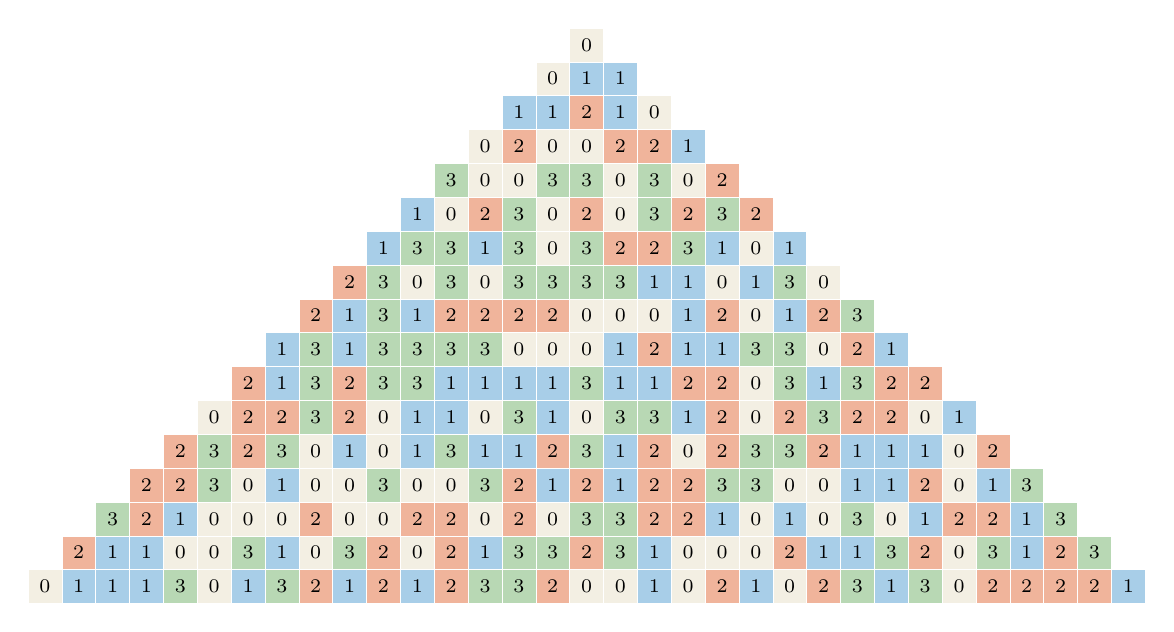
\begin{tikzpicture}[x=0.43cm,y=0.43cm]
\filldraw[fill=color0,draw=white,line width=0.2pt] (0,0) rectangle ++(1,1);
\node[font=\scriptsize] at (0.5,0.5) {0};
\filldraw[fill=color0,draw=white,line width=0.2pt] (-1,-1) rectangle ++(1,1);
\node[font=\scriptsize] at (-0.5,-0.5) {0};
\filldraw[fill=color1,draw=white,line width=0.2pt] (0,-1) rectangle ++(1,1);
\node[font=\scriptsize] at (0.5,-0.5) {1};
\filldraw[fill=color1,draw=white,line width=0.2pt] (1,-1) rectangle ++(1,1);
\node[font=\scriptsize] at (1.5,-0.5) {1};
\filldraw[fill=color1,draw=white,line width=0.2pt] (-2,-2) rectangle ++(1,1);
\node[font=\scriptsize] at (-1.5,-1.5) {1};
\filldraw[fill=color1,draw=white,line width=0.2pt] (-1,-2) rectangle ++(1,1);
\node[font=\scriptsize] at (-0.5,-1.5) {1};
\filldraw[fill=color2,draw=white,line width=0.2pt] (0,-2) rectangle ++(1,1);
\node[font=\scriptsize] at (0.5,-1.5) {2};
\filldraw[fill=color1,draw=white,line width=0.2pt] (1,-2) rectangle ++(1,1);
\node[font=\scriptsize] at (1.5,-1.5) {1};
\filldraw[fill=color0,draw=white,line width=0.2pt] (2,-2) rectangle ++(1,1);
\node[font=\scriptsize] at (2.5,-1.5) {0};
\filldraw[fill=color0,draw=white,line width=0.2pt] (-3,-3) rectangle ++(1,1);
\node[font=\scriptsize] at (-2.5,-2.5) {0};
\filldraw[fill=color2,draw=white,line width=0.2pt] (-2,-3) rectangle ++(1,1);
\node[font=\scriptsize] at (-1.5,-2.5) {2};
\filldraw[fill=color0,draw=white,line width=0.2pt] (-1,-3) rectangle ++(1,1);
\node[font=\scriptsize] at (-0.5,-2.5) {0};
\filldraw[fill=color0,draw=white,line width=0.2pt] (0,-3) rectangle ++(1,1);
\node[font=\scriptsize] at (0.5,-2.5) {0};
\filldraw[fill=color2,draw=white,line width=0.2pt] (1,-3) rectangle ++(1,1);
\node[font=\scriptsize] at (1.5,-2.5) {2};
\filldraw[fill=color2,draw=white,line width=0.2pt] (2,-3) rectangle ++(1,1);
\node[font=\scriptsize] at (2.5,-2.5) {2};
\filldraw[fill=color1,draw=white,line width=0.2pt] (3,-3) rectangle ++(1,1);
\node[font=\scriptsize] at (3.5,-2.5) {1};
\filldraw[fill=color3,draw=white,line width=0.2pt] (-4,-4) rectangle ++(1,1);
\node[font=\scriptsize] at (-3.5,-3.5) {3};
\filldraw[fill=color0,draw=white,line width=0.2pt] (-3,-4) rectangle ++(1,1);
\node[font=\scriptsize] at (-2.5,-3.5) {0};
\filldraw[fill=color0,draw=white,line width=0.2pt] (-2,-4) rectangle ++(1,1);
\node[font=\scriptsize] at (-1.5,-3.5) {0};
\filldraw[fill=color3,draw=white,line width=0.2pt] (-1,-4) rectangle ++(1,1);
\node[font=\scriptsize] at (-0.5,-3.5) {3};
\filldraw[fill=color3,draw=white,line width=0.2pt] (0,-4) rectangle ++(1,1);
\node[font=\scriptsize] at (0.5,-3.5) {3};
\filldraw[fill=color0,draw=white,line width=0.2pt] (1,-4) rectangle ++(1,1);
\node[font=\scriptsize] at (1.5,-3.5) {0};
\filldraw[fill=color3,draw=white,line width=0.2pt] (2,-4) rectangle ++(1,1);
\node[font=\scriptsize] at (2.5,-3.5) {3};
\filldraw[fill=color0,draw=white,line width=0.2pt] (3,-4) rectangle ++(1,1);
\node[font=\scriptsize] at (3.5,-3.5) {0};
\filldraw[fill=color2,draw=white,line width=0.2pt] (4,-4) rectangle ++(1,1);
\node[font=\scriptsize] at (4.5,-3.5) {2};
\filldraw[fill=color1,draw=white,line width=0.2pt] (-5,-5) rectangle ++(1,1);
\node[font=\scriptsize] at (-4.5,-4.5) {1};
\filldraw[fill=color0,draw=white,line width=0.2pt] (-4,-5) rectangle ++(1,1);
\node[font=\scriptsize] at (-3.5,-4.5) {0};
\filldraw[fill=color2,draw=white,line width=0.2pt] (-3,-5) rectangle ++(1,1);
\node[font=\scriptsize] at (-2.5,-4.5) {2};
\filldraw[fill=color3,draw=white,line width=0.2pt] (-2,-5) rectangle ++(1,1);
\node[font=\scriptsize] at (-1.5,-4.5) {3};
\filldraw[fill=color0,draw=white,line width=0.2pt] (-1,-5) rectangle ++(1,1);
\node[font=\scriptsize] at (-0.5,-4.5) {0};
\filldraw[fill=color2,draw=white,line width=0.2pt] (0,-5) rectangle ++(1,1);
\node[font=\scriptsize] at (0.5,-4.5) {2};
\filldraw[fill=color0,draw=white,line width=0.2pt] (1,-5) rectangle ++(1,1);
\node[font=\scriptsize] at (1.5,-4.5) {0};
\filldraw[fill=color3,draw=white,line width=0.2pt] (2,-5) rectangle ++(1,1);
\node[font=\scriptsize] at (2.5,-4.5) {3};
\filldraw[fill=color2,draw=white,line width=0.2pt] (3,-5) rectangle ++(1,1);
\node[font=\scriptsize] at (3.5,-4.5) {2};
\filldraw[fill=color3,draw=white,line width=0.2pt] (4,-5) rectangle ++(1,1);
\node[font=\scriptsize] at (4.5,-4.5) {3};
\filldraw[fill=color2,draw=white,line width=0.2pt] (5,-5) rectangle ++(1,1);
\node[font=\scriptsize] at (5.5,-4.5) {2};
\filldraw[fill=color1,draw=white,line width=0.2pt] (-6,-6) rectangle ++(1,1);
\node[font=\scriptsize] at (-5.5,-5.5) {1};
\filldraw[fill=color3,draw=white,line width=0.2pt] (-5,-6) rectangle ++(1,1);
\node[font=\scriptsize] at (-4.5,-5.5) {3};
\filldraw[fill=color3,draw=white,line width=0.2pt] (-4,-6) rectangle ++(1,1);
\node[font=\scriptsize] at (-3.5,-5.5) {3};
\filldraw[fill=color1,draw=white,line width=0.2pt] (-3,-6) rectangle ++(1,1);
\node[font=\scriptsize] at (-2.5,-5.5) {1};
\filldraw[fill=color3,draw=white,line width=0.2pt] (-2,-6) rectangle ++(1,1);
\node[font=\scriptsize] at (-1.5,-5.5) {3};
\filldraw[fill=color0,draw=white,line width=0.2pt] (-1,-6) rectangle ++(1,1);
\node[font=\scriptsize] at (-0.5,-5.5) {0};
\filldraw[fill=color3,draw=white,line width=0.2pt] (0,-6) rectangle ++(1,1);
\node[font=\scriptsize] at (0.5,-5.5) {3};
\filldraw[fill=color2,draw=white,line width=0.2pt] (1,-6) rectangle ++(1,1);
\node[font=\scriptsize] at (1.5,-5.5) {2};
\filldraw[fill=color2,draw=white,line width=0.2pt] (2,-6) rectangle ++(1,1);
\node[font=\scriptsize] at (2.5,-5.5) {2};
\filldraw[fill=color3,draw=white,line width=0.2pt] (3,-6) rectangle ++(1,1);
\node[font=\scriptsize] at (3.5,-5.5) {3};
\filldraw[fill=color1,draw=white,line width=0.2pt] (4,-6) rectangle ++(1,1);
\node[font=\scriptsize] at (4.5,-5.5) {1};
\filldraw[fill=color0,draw=white,line width=0.2pt] (5,-6) rectangle ++(1,1);
\node[font=\scriptsize] at (5.5,-5.5) {0};
\filldraw[fill=color1,draw=white,line width=0.2pt] (6,-6) rectangle ++(1,1);
\node[font=\scriptsize] at (6.5,-5.5) {1};
\filldraw[fill=color2,draw=white,line width=0.2pt] (-7,-7) rectangle ++(1,1);
\node[font=\scriptsize] at (-6.5,-6.5) {2};
\filldraw[fill=color3,draw=white,line width=0.2pt] (-6,-7) rectangle ++(1,1);
\node[font=\scriptsize] at (-5.5,-6.5) {3};
\filldraw[fill=color0,draw=white,line width=0.2pt] (-5,-7) rectangle ++(1,1);
\node[font=\scriptsize] at (-4.5,-6.5) {0};
\filldraw[fill=color3,draw=white,line width=0.2pt] (-4,-7) rectangle ++(1,1);
\node[font=\scriptsize] at (-3.5,-6.5) {3};
\filldraw[fill=color0,draw=white,line width=0.2pt] (-3,-7) rectangle ++(1,1);
\node[font=\scriptsize] at (-2.5,-6.5) {0};
\filldraw[fill=color3,draw=white,line width=0.2pt] (-2,-7) rectangle ++(1,1);
\node[font=\scriptsize] at (-1.5,-6.5) {3};
\filldraw[fill=color3,draw=white,line width=0.2pt] (-1,-7) rectangle ++(1,1);
\node[font=\scriptsize] at (-0.5,-6.5) {3};
\filldraw[fill=color3,draw=white,line width=0.2pt] (0,-7) rectangle ++(1,1);
\node[font=\scriptsize] at (0.5,-6.5) {3};
\filldraw[fill=color3,draw=white,line width=0.2pt] (1,-7) rectangle ++(1,1);
\node[font=\scriptsize] at (1.5,-6.5) {3};
\filldraw[fill=color1,draw=white,line width=0.2pt] (2,-7) rectangle ++(1,1);
\node[font=\scriptsize] at (2.5,-6.5) {1};
\filldraw[fill=color1,draw=white,line width=0.2pt] (3,-7) rectangle ++(1,1);
\node[font=\scriptsize] at (3.5,-6.5) {1};
\filldraw[fill=color0,draw=white,line width=0.2pt] (4,-7) rectangle ++(1,1);
\node[font=\scriptsize] at (4.5,-6.5) {0};
\filldraw[fill=color1,draw=white,line width=0.2pt] (5,-7) rectangle ++(1,1);
\node[font=\scriptsize] at (5.5,-6.5) {1};
\filldraw[fill=color3,draw=white,line width=0.2pt] (6,-7) rectangle ++(1,1);
\node[font=\scriptsize] at (6.5,-6.5) {3};
\filldraw[fill=color0,draw=white,line width=0.2pt] (7,-7) rectangle ++(1,1);
\node[font=\scriptsize] at (7.5,-6.5) {0};
\filldraw[fill=color2,draw=white,line width=0.2pt] (-8,-8) rectangle ++(1,1);
\node[font=\scriptsize] at (-7.5,-7.5) {2};
\filldraw[fill=color1,draw=white,line width=0.2pt] (-7,-8) rectangle ++(1,1);
\node[font=\scriptsize] at (-6.5,-7.5) {1};
\filldraw[fill=color3,draw=white,line width=0.2pt] (-6,-8) rectangle ++(1,1);
\node[font=\scriptsize] at (-5.5,-7.5) {3};
\filldraw[fill=color1,draw=white,line width=0.2pt] (-5,-8) rectangle ++(1,1);
\node[font=\scriptsize] at (-4.5,-7.5) {1};
\filldraw[fill=color2,draw=white,line width=0.2pt] (-4,-8) rectangle ++(1,1);
\node[font=\scriptsize] at (-3.5,-7.5) {2};
\filldraw[fill=color2,draw=white,line width=0.2pt] (-3,-8) rectangle ++(1,1);
\node[font=\scriptsize] at (-2.5,-7.5) {2};
\filldraw[fill=color2,draw=white,line width=0.2pt] (-2,-8) rectangle ++(1,1);
\node[font=\scriptsize] at (-1.5,-7.5) {2};
\filldraw[fill=color2,draw=white,line width=0.2pt] (-1,-8) rectangle ++(1,1);
\node[font=\scriptsize] at (-0.5,-7.5) {2};
\filldraw[fill=color0,draw=white,line width=0.2pt] (0,-8) rectangle ++(1,1);
\node[font=\scriptsize] at (0.5,-7.5) {0};
\filldraw[fill=color0,draw=white,line width=0.2pt] (1,-8) rectangle ++(1,1);
\node[font=\scriptsize] at (1.5,-7.5) {0};
\filldraw[fill=color0,draw=white,line width=0.2pt] (2,-8) rectangle ++(1,1);
\node[font=\scriptsize] at (2.5,-7.5) {0};
\filldraw[fill=color1,draw=white,line width=0.2pt] (3,-8) rectangle ++(1,1);
\node[font=\scriptsize] at (3.5,-7.5) {1};
\filldraw[fill=color2,draw=white,line width=0.2pt] (4,-8) rectangle ++(1,1);
\node[font=\scriptsize] at (4.5,-7.5) {2};
\filldraw[fill=color0,draw=white,line width=0.2pt] (5,-8) rectangle ++(1,1);
\node[font=\scriptsize] at (5.5,-7.5) {0};
\filldraw[fill=color1,draw=white,line width=0.2pt] (6,-8) rectangle ++(1,1);
\node[font=\scriptsize] at (6.5,-7.5) {1};
\filldraw[fill=color2,draw=white,line width=0.2pt] (7,-8) rectangle ++(1,1);
\node[font=\scriptsize] at (7.5,-7.5) {2};
\filldraw[fill=color3,draw=white,line width=0.2pt] (8,-8) rectangle ++(1,1);
\node[font=\scriptsize] at (8.5,-7.5) {3};
\filldraw[fill=color1,draw=white,line width=0.2pt] (-9,-9) rectangle ++(1,1);
\node[font=\scriptsize] at (-8.5,-8.5) {1};
\filldraw[fill=color3,draw=white,line width=0.2pt] (-8,-9) rectangle ++(1,1);
\node[font=\scriptsize] at (-7.5,-8.5) {3};
\filldraw[fill=color1,draw=white,line width=0.2pt] (-7,-9) rectangle ++(1,1);
\node[font=\scriptsize] at (-6.5,-8.5) {1};
\filldraw[fill=color3,draw=white,line width=0.2pt] (-6,-9) rectangle ++(1,1);
\node[font=\scriptsize] at (-5.5,-8.5) {3};
\filldraw[fill=color3,draw=white,line width=0.2pt] (-5,-9) rectangle ++(1,1);
\node[font=\scriptsize] at (-4.5,-8.5) {3};
\filldraw[fill=color3,draw=white,line width=0.2pt] (-4,-9) rectangle ++(1,1);
\node[font=\scriptsize] at (-3.5,-8.5) {3};
\filldraw[fill=color3,draw=white,line width=0.2pt] (-3,-9) rectangle ++(1,1);
\node[font=\scriptsize] at (-2.5,-8.5) {3};
\filldraw[fill=color0,draw=white,line width=0.2pt] (-2,-9) rectangle ++(1,1);
\node[font=\scriptsize] at (-1.5,-8.5) {0};
\filldraw[fill=color0,draw=white,line width=0.2pt] (-1,-9) rectangle ++(1,1);
\node[font=\scriptsize] at (-0.5,-8.5) {0};
\filldraw[fill=color0,draw=white,line width=0.2pt] (0,-9) rectangle ++(1,1);
\node[font=\scriptsize] at (0.5,-8.5) {0};
\filldraw[fill=color1,draw=white,line width=0.2pt] (1,-9) rectangle ++(1,1);
\node[font=\scriptsize] at (1.5,-8.5) {1};
\filldraw[fill=color2,draw=white,line width=0.2pt] (2,-9) rectangle ++(1,1);
\node[font=\scriptsize] at (2.5,-8.5) {2};
\filldraw[fill=color1,draw=white,line width=0.2pt] (3,-9) rectangle ++(1,1);
\node[font=\scriptsize] at (3.5,-8.5) {1};
\filldraw[fill=color1,draw=white,line width=0.2pt] (4,-9) rectangle ++(1,1);
\node[font=\scriptsize] at (4.5,-8.5) {1};
\filldraw[fill=color3,draw=white,line width=0.2pt] (5,-9) rectangle ++(1,1);
\node[font=\scriptsize] at (5.5,-8.5) {3};
\filldraw[fill=color3,draw=white,line width=0.2pt] (6,-9) rectangle ++(1,1);
\node[font=\scriptsize] at (6.5,-8.5) {3};
\filldraw[fill=color0,draw=white,line width=0.2pt] (7,-9) rectangle ++(1,1);
\node[font=\scriptsize] at (7.5,-8.5) {0};
\filldraw[fill=color2,draw=white,line width=0.2pt] (8,-9) rectangle ++(1,1);
\node[font=\scriptsize] at (8.5,-8.5) {2};
\filldraw[fill=color1,draw=white,line width=0.2pt] (9,-9) rectangle ++(1,1);
\node[font=\scriptsize] at (9.5,-8.5) {1};
\filldraw[fill=color2,draw=white,line width=0.2pt] (-10,-10) rectangle ++(1,1);
\node[font=\scriptsize] at (-9.5,-9.5) {2};
\filldraw[fill=color1,draw=white,line width=0.2pt] (-9,-10) rectangle ++(1,1);
\node[font=\scriptsize] at (-8.5,-9.5) {1};
\filldraw[fill=color3,draw=white,line width=0.2pt] (-8,-10) rectangle ++(1,1);
\node[font=\scriptsize] at (-7.5,-9.5) {3};
\filldraw[fill=color2,draw=white,line width=0.2pt] (-7,-10) rectangle ++(1,1);
\node[font=\scriptsize] at (-6.5,-9.5) {2};
\filldraw[fill=color3,draw=white,line width=0.2pt] (-6,-10) rectangle ++(1,1);
\node[font=\scriptsize] at (-5.5,-9.5) {3};
\filldraw[fill=color3,draw=white,line width=0.2pt] (-5,-10) rectangle ++(1,1);
\node[font=\scriptsize] at (-4.5,-9.5) {3};
\filldraw[fill=color1,draw=white,line width=0.2pt] (-4,-10) rectangle ++(1,1);
\node[font=\scriptsize] at (-3.5,-9.5) {1};
\filldraw[fill=color1,draw=white,line width=0.2pt] (-3,-10) rectangle ++(1,1);
\node[font=\scriptsize] at (-2.5,-9.5) {1};
\filldraw[fill=color1,draw=white,line width=0.2pt] (-2,-10) rectangle ++(1,1);
\node[font=\scriptsize] at (-1.5,-9.5) {1};
\filldraw[fill=color1,draw=white,line width=0.2pt] (-1,-10) rectangle ++(1,1);
\node[font=\scriptsize] at (-0.5,-9.5) {1};
\filldraw[fill=color3,draw=white,line width=0.2pt] (0,-10) rectangle ++(1,1);
\node[font=\scriptsize] at (0.5,-9.5) {3};
\filldraw[fill=color1,draw=white,line width=0.2pt] (1,-10) rectangle ++(1,1);
\node[font=\scriptsize] at (1.5,-9.5) {1};
\filldraw[fill=color1,draw=white,line width=0.2pt] (2,-10) rectangle ++(1,1);
\node[font=\scriptsize] at (2.5,-9.5) {1};
\filldraw[fill=color2,draw=white,line width=0.2pt] (3,-10) rectangle ++(1,1);
\node[font=\scriptsize] at (3.5,-9.5) {2};
\filldraw[fill=color2,draw=white,line width=0.2pt] (4,-10) rectangle ++(1,1);
\node[font=\scriptsize] at (4.5,-9.5) {2};
\filldraw[fill=color0,draw=white,line width=0.2pt] (5,-10) rectangle ++(1,1);
\node[font=\scriptsize] at (5.5,-9.5) {0};
\filldraw[fill=color3,draw=white,line width=0.2pt] (6,-10) rectangle ++(1,1);
\node[font=\scriptsize] at (6.5,-9.5) {3};
\filldraw[fill=color1,draw=white,line width=0.2pt] (7,-10) rectangle ++(1,1);
\node[font=\scriptsize] at (7.5,-9.5) {1};
\filldraw[fill=color3,draw=white,line width=0.2pt] (8,-10) rectangle ++(1,1);
\node[font=\scriptsize] at (8.5,-9.5) {3};
\filldraw[fill=color2,draw=white,line width=0.2pt] (9,-10) rectangle ++(1,1);
\node[font=\scriptsize] at (9.5,-9.5) {2};
\filldraw[fill=color2,draw=white,line width=0.2pt] (10,-10) rectangle ++(1,1);
\node[font=\scriptsize] at (10.5,-9.5) {2};
\filldraw[fill=color0,draw=white,line width=0.2pt] (-11,-11) rectangle ++(1,1);
\node[font=\scriptsize] at (-10.5,-10.5) {0};
\filldraw[fill=color2,draw=white,line width=0.2pt] (-10,-11) rectangle ++(1,1);
\node[font=\scriptsize] at (-9.5,-10.5) {2};
\filldraw[fill=color2,draw=white,line width=0.2pt] (-9,-11) rectangle ++(1,1);
\node[font=\scriptsize] at (-8.5,-10.5) {2};
\filldraw[fill=color3,draw=white,line width=0.2pt] (-8,-11) rectangle ++(1,1);
\node[font=\scriptsize] at (-7.5,-10.5) {3};
\filldraw[fill=color2,draw=white,line width=0.2pt] (-7,-11) rectangle ++(1,1);
\node[font=\scriptsize] at (-6.5,-10.5) {2};
\filldraw[fill=color0,draw=white,line width=0.2pt] (-6,-11) rectangle ++(1,1);
\node[font=\scriptsize] at (-5.5,-10.5) {0};
\filldraw[fill=color1,draw=white,line width=0.2pt] (-5,-11) rectangle ++(1,1);
\node[font=\scriptsize] at (-4.5,-10.5) {1};
\filldraw[fill=color1,draw=white,line width=0.2pt] (-4,-11) rectangle ++(1,1);
\node[font=\scriptsize] at (-3.5,-10.5) {1};
\filldraw[fill=color0,draw=white,line width=0.2pt] (-3,-11) rectangle ++(1,1);
\node[font=\scriptsize] at (-2.5,-10.5) {0};
\filldraw[fill=color3,draw=white,line width=0.2pt] (-2,-11) rectangle ++(1,1);
\node[font=\scriptsize] at (-1.5,-10.5) {3};
\filldraw[fill=color1,draw=white,line width=0.2pt] (-1,-11) rectangle ++(1,1);
\node[font=\scriptsize] at (-0.5,-10.5) {1};
\filldraw[fill=color0,draw=white,line width=0.2pt] (0,-11) rectangle ++(1,1);
\node[font=\scriptsize] at (0.5,-10.5) {0};
\filldraw[fill=color3,draw=white,line width=0.2pt] (1,-11) rectangle ++(1,1);
\node[font=\scriptsize] at (1.5,-10.5) {3};
\filldraw[fill=color3,draw=white,line width=0.2pt] (2,-11) rectangle ++(1,1);
\node[font=\scriptsize] at (2.5,-10.5) {3};
\filldraw[fill=color1,draw=white,line width=0.2pt] (3,-11) rectangle ++(1,1);
\node[font=\scriptsize] at (3.5,-10.5) {1};
\filldraw[fill=color2,draw=white,line width=0.2pt] (4,-11) rectangle ++(1,1);
\node[font=\scriptsize] at (4.5,-10.5) {2};
\filldraw[fill=color0,draw=white,line width=0.2pt] (5,-11) rectangle ++(1,1);
\node[font=\scriptsize] at (5.5,-10.5) {0};
\filldraw[fill=color2,draw=white,line width=0.2pt] (6,-11) rectangle ++(1,1);
\node[font=\scriptsize] at (6.5,-10.5) {2};
\filldraw[fill=color3,draw=white,line width=0.2pt] (7,-11) rectangle ++(1,1);
\node[font=\scriptsize] at (7.5,-10.5) {3};
\filldraw[fill=color2,draw=white,line width=0.2pt] (8,-11) rectangle ++(1,1);
\node[font=\scriptsize] at (8.5,-10.5) {2};
\filldraw[fill=color2,draw=white,line width=0.2pt] (9,-11) rectangle ++(1,1);
\node[font=\scriptsize] at (9.5,-10.5) {2};
\filldraw[fill=color0,draw=white,line width=0.2pt] (10,-11) rectangle ++(1,1);
\node[font=\scriptsize] at (10.5,-10.5) {0};
\filldraw[fill=color1,draw=white,line width=0.2pt] (11,-11) rectangle ++(1,1);
\node[font=\scriptsize] at (11.5,-10.5) {1};
\filldraw[fill=color2,draw=white,line width=0.2pt] (-12,-12) rectangle ++(1,1);
\node[font=\scriptsize] at (-11.5,-11.5) {2};
\filldraw[fill=color3,draw=white,line width=0.2pt] (-11,-12) rectangle ++(1,1);
\node[font=\scriptsize] at (-10.5,-11.5) {3};
\filldraw[fill=color2,draw=white,line width=0.2pt] (-10,-12) rectangle ++(1,1);
\node[font=\scriptsize] at (-9.5,-11.5) {2};
\filldraw[fill=color3,draw=white,line width=0.2pt] (-9,-12) rectangle ++(1,1);
\node[font=\scriptsize] at (-8.5,-11.5) {3};
\filldraw[fill=color0,draw=white,line width=0.2pt] (-8,-12) rectangle ++(1,1);
\node[font=\scriptsize] at (-7.5,-11.5) {0};
\filldraw[fill=color1,draw=white,line width=0.2pt] (-7,-12) rectangle ++(1,1);
\node[font=\scriptsize] at (-6.5,-11.5) {1};
\filldraw[fill=color0,draw=white,line width=0.2pt] (-6,-12) rectangle ++(1,1);
\node[font=\scriptsize] at (-5.5,-11.5) {0};
\filldraw[fill=color1,draw=white,line width=0.2pt] (-5,-12) rectangle ++(1,1);
\node[font=\scriptsize] at (-4.5,-11.5) {1};
\filldraw[fill=color3,draw=white,line width=0.2pt] (-4,-12) rectangle ++(1,1);
\node[font=\scriptsize] at (-3.5,-11.5) {3};
\filldraw[fill=color1,draw=white,line width=0.2pt] (-3,-12) rectangle ++(1,1);
\node[font=\scriptsize] at (-2.5,-11.5) {1};
\filldraw[fill=color1,draw=white,line width=0.2pt] (-2,-12) rectangle ++(1,1);
\node[font=\scriptsize] at (-1.5,-11.5) {1};
\filldraw[fill=color2,draw=white,line width=0.2pt] (-1,-12) rectangle ++(1,1);
\node[font=\scriptsize] at (-0.5,-11.5) {2};
\filldraw[fill=color3,draw=white,line width=0.2pt] (0,-12) rectangle ++(1,1);
\node[font=\scriptsize] at (0.5,-11.5) {3};
\filldraw[fill=color1,draw=white,line width=0.2pt] (1,-12) rectangle ++(1,1);
\node[font=\scriptsize] at (1.5,-11.5) {1};
\filldraw[fill=color2,draw=white,line width=0.2pt] (2,-12) rectangle ++(1,1);
\node[font=\scriptsize] at (2.5,-11.5) {2};
\filldraw[fill=color0,draw=white,line width=0.2pt] (3,-12) rectangle ++(1,1);
\node[font=\scriptsize] at (3.5,-11.5) {0};
\filldraw[fill=color2,draw=white,line width=0.2pt] (4,-12) rectangle ++(1,1);
\node[font=\scriptsize] at (4.5,-11.5) {2};
\filldraw[fill=color3,draw=white,line width=0.2pt] (5,-12) rectangle ++(1,1);
\node[font=\scriptsize] at (5.5,-11.5) {3};
\filldraw[fill=color3,draw=white,line width=0.2pt] (6,-12) rectangle ++(1,1);
\node[font=\scriptsize] at (6.5,-11.5) {3};
\filldraw[fill=color2,draw=white,line width=0.2pt] (7,-12) rectangle ++(1,1);
\node[font=\scriptsize] at (7.5,-11.5) {2};
\filldraw[fill=color1,draw=white,line width=0.2pt] (8,-12) rectangle ++(1,1);
\node[font=\scriptsize] at (8.5,-11.5) {1};
\filldraw[fill=color1,draw=white,line width=0.2pt] (9,-12) rectangle ++(1,1);
\node[font=\scriptsize] at (9.5,-11.5) {1};
\filldraw[fill=color1,draw=white,line width=0.2pt] (10,-12) rectangle ++(1,1);
\node[font=\scriptsize] at (10.5,-11.5) {1};
\filldraw[fill=color0,draw=white,line width=0.2pt] (11,-12) rectangle ++(1,1);
\node[font=\scriptsize] at (11.5,-11.5) {0};
\filldraw[fill=color2,draw=white,line width=0.2pt] (12,-12) rectangle ++(1,1);
\node[font=\scriptsize] at (12.5,-11.5) {2};
\filldraw[fill=color2,draw=white,line width=0.2pt] (-13,-13) rectangle ++(1,1);
\node[font=\scriptsize] at (-12.5,-12.5) {2};
\filldraw[fill=color2,draw=white,line width=0.2pt] (-12,-13) rectangle ++(1,1);
\node[font=\scriptsize] at (-11.5,-12.5) {2};
\filldraw[fill=color3,draw=white,line width=0.2pt] (-11,-13) rectangle ++(1,1);
\node[font=\scriptsize] at (-10.5,-12.5) {3};
\filldraw[fill=color0,draw=white,line width=0.2pt] (-10,-13) rectangle ++(1,1);
\node[font=\scriptsize] at (-9.5,-12.5) {0};
\filldraw[fill=color1,draw=white,line width=0.2pt] (-9,-13) rectangle ++(1,1);
\node[font=\scriptsize] at (-8.5,-12.5) {1};
\filldraw[fill=color0,draw=white,line width=0.2pt] (-8,-13) rectangle ++(1,1);
\node[font=\scriptsize] at (-7.5,-12.5) {0};
\filldraw[fill=color0,draw=white,line width=0.2pt] (-7,-13) rectangle ++(1,1);
\node[font=\scriptsize] at (-6.5,-12.5) {0};
\filldraw[fill=color3,draw=white,line width=0.2pt] (-6,-13) rectangle ++(1,1);
\node[font=\scriptsize] at (-5.5,-12.5) {3};
\filldraw[fill=color0,draw=white,line width=0.2pt] (-5,-13) rectangle ++(1,1);
\node[font=\scriptsize] at (-4.5,-12.5) {0};
\filldraw[fill=color0,draw=white,line width=0.2pt] (-4,-13) rectangle ++(1,1);
\node[font=\scriptsize] at (-3.5,-12.5) {0};
\filldraw[fill=color3,draw=white,line width=0.2pt] (-3,-13) rectangle ++(1,1);
\node[font=\scriptsize] at (-2.5,-12.5) {3};
\filldraw[fill=color2,draw=white,line width=0.2pt] (-2,-13) rectangle ++(1,1);
\node[font=\scriptsize] at (-1.5,-12.5) {2};
\filldraw[fill=color1,draw=white,line width=0.2pt] (-1,-13) rectangle ++(1,1);
\node[font=\scriptsize] at (-0.5,-12.5) {1};
\filldraw[fill=color2,draw=white,line width=0.2pt] (0,-13) rectangle ++(1,1);
\node[font=\scriptsize] at (0.5,-12.5) {2};
\filldraw[fill=color1,draw=white,line width=0.2pt] (1,-13) rectangle ++(1,1);
\node[font=\scriptsize] at (1.5,-12.5) {1};
\filldraw[fill=color2,draw=white,line width=0.2pt] (2,-13) rectangle ++(1,1);
\node[font=\scriptsize] at (2.5,-12.5) {2};
\filldraw[fill=color2,draw=white,line width=0.2pt] (3,-13) rectangle ++(1,1);
\node[font=\scriptsize] at (3.5,-12.5) {2};
\filldraw[fill=color3,draw=white,line width=0.2pt] (4,-13) rectangle ++(1,1);
\node[font=\scriptsize] at (4.5,-12.5) {3};
\filldraw[fill=color3,draw=white,line width=0.2pt] (5,-13) rectangle ++(1,1);
\node[font=\scriptsize] at (5.5,-12.5) {3};
\filldraw[fill=color0,draw=white,line width=0.2pt] (6,-13) rectangle ++(1,1);
\node[font=\scriptsize] at (6.5,-12.5) {0};
\filldraw[fill=color0,draw=white,line width=0.2pt] (7,-13) rectangle ++(1,1);
\node[font=\scriptsize] at (7.5,-12.5) {0};
\filldraw[fill=color1,draw=white,line width=0.2pt] (8,-13) rectangle ++(1,1);
\node[font=\scriptsize] at (8.5,-12.5) {1};
\filldraw[fill=color1,draw=white,line width=0.2pt] (9,-13) rectangle ++(1,1);
\node[font=\scriptsize] at (9.5,-12.5) {1};
\filldraw[fill=color2,draw=white,line width=0.2pt] (10,-13) rectangle ++(1,1);
\node[font=\scriptsize] at (10.5,-12.5) {2};
\filldraw[fill=color0,draw=white,line width=0.2pt] (11,-13) rectangle ++(1,1);
\node[font=\scriptsize] at (11.5,-12.5) {0};
\filldraw[fill=color1,draw=white,line width=0.2pt] (12,-13) rectangle ++(1,1);
\node[font=\scriptsize] at (12.5,-12.5) {1};
\filldraw[fill=color3,draw=white,line width=0.2pt] (13,-13) rectangle ++(1,1);
\node[font=\scriptsize] at (13.5,-12.5) {3};
\filldraw[fill=color3,draw=white,line width=0.2pt] (-14,-14) rectangle ++(1,1);
\node[font=\scriptsize] at (-13.5,-13.5) {3};
\filldraw[fill=color2,draw=white,line width=0.2pt] (-13,-14) rectangle ++(1,1);
\node[font=\scriptsize] at (-12.5,-13.5) {2};
\filldraw[fill=color1,draw=white,line width=0.2pt] (-12,-14) rectangle ++(1,1);
\node[font=\scriptsize] at (-11.5,-13.5) {1};
\filldraw[fill=color0,draw=white,line width=0.2pt] (-11,-14) rectangle ++(1,1);
\node[font=\scriptsize] at (-10.5,-13.5) {0};
\filldraw[fill=color0,draw=white,line width=0.2pt] (-10,-14) rectangle ++(1,1);
\node[font=\scriptsize] at (-9.5,-13.5) {0};
\filldraw[fill=color0,draw=white,line width=0.2pt] (-9,-14) rectangle ++(1,1);
\node[font=\scriptsize] at (-8.5,-13.5) {0};
\filldraw[fill=color2,draw=white,line width=0.2pt] (-8,-14) rectangle ++(1,1);
\node[font=\scriptsize] at (-7.5,-13.5) {2};
\filldraw[fill=color0,draw=white,line width=0.2pt] (-7,-14) rectangle ++(1,1);
\node[font=\scriptsize] at (-6.5,-13.5) {0};
\filldraw[fill=color0,draw=white,line width=0.2pt] (-6,-14) rectangle ++(1,1);
\node[font=\scriptsize] at (-5.5,-13.5) {0};
\filldraw[fill=color2,draw=white,line width=0.2pt] (-5,-14) rectangle ++(1,1);
\node[font=\scriptsize] at (-4.5,-13.5) {2};
\filldraw[fill=color2,draw=white,line width=0.2pt] (-4,-14) rectangle ++(1,1);
\node[font=\scriptsize] at (-3.5,-13.5) {2};
\filldraw[fill=color0,draw=white,line width=0.2pt] (-3,-14) rectangle ++(1,1);
\node[font=\scriptsize] at (-2.5,-13.5) {0};
\filldraw[fill=color2,draw=white,line width=0.2pt] (-2,-14) rectangle ++(1,1);
\node[font=\scriptsize] at (-1.5,-13.5) {2};
\filldraw[fill=color0,draw=white,line width=0.2pt] (-1,-14) rectangle ++(1,1);
\node[font=\scriptsize] at (-0.5,-13.5) {0};
\filldraw[fill=color3,draw=white,line width=0.2pt] (0,-14) rectangle ++(1,1);
\node[font=\scriptsize] at (0.5,-13.5) {3};
\filldraw[fill=color3,draw=white,line width=0.2pt] (1,-14) rectangle ++(1,1);
\node[font=\scriptsize] at (1.5,-13.5) {3};
\filldraw[fill=color2,draw=white,line width=0.2pt] (2,-14) rectangle ++(1,1);
\node[font=\scriptsize] at (2.5,-13.5) {2};
\filldraw[fill=color2,draw=white,line width=0.2pt] (3,-14) rectangle ++(1,1);
\node[font=\scriptsize] at (3.5,-13.5) {2};
\filldraw[fill=color1,draw=white,line width=0.2pt] (4,-14) rectangle ++(1,1);
\node[font=\scriptsize] at (4.5,-13.5) {1};
\filldraw[fill=color0,draw=white,line width=0.2pt] (5,-14) rectangle ++(1,1);
\node[font=\scriptsize] at (5.5,-13.5) {0};
\filldraw[fill=color1,draw=white,line width=0.2pt] (6,-14) rectangle ++(1,1);
\node[font=\scriptsize] at (6.5,-13.5) {1};
\filldraw[fill=color0,draw=white,line width=0.2pt] (7,-14) rectangle ++(1,1);
\node[font=\scriptsize] at (7.5,-13.5) {0};
\filldraw[fill=color3,draw=white,line width=0.2pt] (8,-14) rectangle ++(1,1);
\node[font=\scriptsize] at (8.5,-13.5) {3};
\filldraw[fill=color0,draw=white,line width=0.2pt] (9,-14) rectangle ++(1,1);
\node[font=\scriptsize] at (9.5,-13.5) {0};
\filldraw[fill=color1,draw=white,line width=0.2pt] (10,-14) rectangle ++(1,1);
\node[font=\scriptsize] at (10.5,-13.5) {1};
\filldraw[fill=color2,draw=white,line width=0.2pt] (11,-14) rectangle ++(1,1);
\node[font=\scriptsize] at (11.5,-13.5) {2};
\filldraw[fill=color2,draw=white,line width=0.2pt] (12,-14) rectangle ++(1,1);
\node[font=\scriptsize] at (12.5,-13.5) {2};
\filldraw[fill=color1,draw=white,line width=0.2pt] (13,-14) rectangle ++(1,1);
\node[font=\scriptsize] at (13.5,-13.5) {1};
\filldraw[fill=color3,draw=white,line width=0.2pt] (14,-14) rectangle ++(1,1);
\node[font=\scriptsize] at (14.5,-13.5) {3};
\filldraw[fill=color2,draw=white,line width=0.2pt] (-15,-15) rectangle ++(1,1);
\node[font=\scriptsize] at (-14.5,-14.5) {2};
\filldraw[fill=color1,draw=white,line width=0.2pt] (-14,-15) rectangle ++(1,1);
\node[font=\scriptsize] at (-13.5,-14.5) {1};
\filldraw[fill=color1,draw=white,line width=0.2pt] (-13,-15) rectangle ++(1,1);
\node[font=\scriptsize] at (-12.5,-14.5) {1};
\filldraw[fill=color0,draw=white,line width=0.2pt] (-12,-15) rectangle ++(1,1);
\node[font=\scriptsize] at (-11.5,-14.5) {0};
\filldraw[fill=color0,draw=white,line width=0.2pt] (-11,-15) rectangle ++(1,1);
\node[font=\scriptsize] at (-10.5,-14.5) {0};
\filldraw[fill=color3,draw=white,line width=0.2pt] (-10,-15) rectangle ++(1,1);
\node[font=\scriptsize] at (-9.5,-14.5) {3};
\filldraw[fill=color1,draw=white,line width=0.2pt] (-9,-15) rectangle ++(1,1);
\node[font=\scriptsize] at (-8.5,-14.5) {1};
\filldraw[fill=color0,draw=white,line width=0.2pt] (-8,-15) rectangle ++(1,1);
\node[font=\scriptsize] at (-7.5,-14.5) {0};
\filldraw[fill=color3,draw=white,line width=0.2pt] (-7,-15) rectangle ++(1,1);
\node[font=\scriptsize] at (-6.5,-14.5) {3};
\filldraw[fill=color2,draw=white,line width=0.2pt] (-6,-15) rectangle ++(1,1);
\node[font=\scriptsize] at (-5.5,-14.5) {2};
\filldraw[fill=color0,draw=white,line width=0.2pt] (-5,-15) rectangle ++(1,1);
\node[font=\scriptsize] at (-4.5,-14.5) {0};
\filldraw[fill=color2,draw=white,line width=0.2pt] (-4,-15) rectangle ++(1,1);
\node[font=\scriptsize] at (-3.5,-14.5) {2};
\filldraw[fill=color1,draw=white,line width=0.2pt] (-3,-15) rectangle ++(1,1);
\node[font=\scriptsize] at (-2.5,-14.5) {1};
\filldraw[fill=color3,draw=white,line width=0.2pt] (-2,-15) rectangle ++(1,1);
\node[font=\scriptsize] at (-1.5,-14.5) {3};
\filldraw[fill=color3,draw=white,line width=0.2pt] (-1,-15) rectangle ++(1,1);
\node[font=\scriptsize] at (-0.5,-14.5) {3};
\filldraw[fill=color2,draw=white,line width=0.2pt] (0,-15) rectangle ++(1,1);
\node[font=\scriptsize] at (0.5,-14.5) {2};
\filldraw[fill=color3,draw=white,line width=0.2pt] (1,-15) rectangle ++(1,1);
\node[font=\scriptsize] at (1.5,-14.5) {3};
\filldraw[fill=color1,draw=white,line width=0.2pt] (2,-15) rectangle ++(1,1);
\node[font=\scriptsize] at (2.5,-14.5) {1};
\filldraw[fill=color0,draw=white,line width=0.2pt] (3,-15) rectangle ++(1,1);
\node[font=\scriptsize] at (3.5,-14.5) {0};
\filldraw[fill=color0,draw=white,line width=0.2pt] (4,-15) rectangle ++(1,1);
\node[font=\scriptsize] at (4.5,-14.5) {0};
\filldraw[fill=color0,draw=white,line width=0.2pt] (5,-15) rectangle ++(1,1);
\node[font=\scriptsize] at (5.5,-14.5) {0};
\filldraw[fill=color2,draw=white,line width=0.2pt] (6,-15) rectangle ++(1,1);
\node[font=\scriptsize] at (6.5,-14.5) {2};
\filldraw[fill=color1,draw=white,line width=0.2pt] (7,-15) rectangle ++(1,1);
\node[font=\scriptsize] at (7.5,-14.5) {1};
\filldraw[fill=color1,draw=white,line width=0.2pt] (8,-15) rectangle ++(1,1);
\node[font=\scriptsize] at (8.5,-14.5) {1};
\filldraw[fill=color3,draw=white,line width=0.2pt] (9,-15) rectangle ++(1,1);
\node[font=\scriptsize] at (9.5,-14.5) {3};
\filldraw[fill=color2,draw=white,line width=0.2pt] (10,-15) rectangle ++(1,1);
\node[font=\scriptsize] at (10.5,-14.5) {2};
\filldraw[fill=color0,draw=white,line width=0.2pt] (11,-15) rectangle ++(1,1);
\node[font=\scriptsize] at (11.5,-14.5) {0};
\filldraw[fill=color3,draw=white,line width=0.2pt] (12,-15) rectangle ++(1,1);
\node[font=\scriptsize] at (12.5,-14.5) {3};
\filldraw[fill=color1,draw=white,line width=0.2pt] (13,-15) rectangle ++(1,1);
\node[font=\scriptsize] at (13.5,-14.5) {1};
\filldraw[fill=color2,draw=white,line width=0.2pt] (14,-15) rectangle ++(1,1);
\node[font=\scriptsize] at (14.5,-14.5) {2};
\filldraw[fill=color3,draw=white,line width=0.2pt] (15,-15) rectangle ++(1,1);
\node[font=\scriptsize] at (15.5,-14.5) {3};
\filldraw[fill=color0,draw=white,line width=0.2pt] (-16,-16) rectangle ++(1,1);
\node[font=\scriptsize] at (-15.5,-15.5) {0};
\filldraw[fill=color1,draw=white,line width=0.2pt] (-15,-16) rectangle ++(1,1);
\node[font=\scriptsize] at (-14.5,-15.5) {1};
\filldraw[fill=color1,draw=white,line width=0.2pt] (-14,-16) rectangle ++(1,1);
\node[font=\scriptsize] at (-13.5,-15.5) {1};
\filldraw[fill=color1,draw=white,line width=0.2pt] (-13,-16) rectangle ++(1,1);
\node[font=\scriptsize] at (-12.5,-15.5) {1};
\filldraw[fill=color3,draw=white,line width=0.2pt] (-12,-16) rectangle ++(1,1);
\node[font=\scriptsize] at (-11.5,-15.5) {3};
\filldraw[fill=color0,draw=white,line width=0.2pt] (-11,-16) rectangle ++(1,1);
\node[font=\scriptsize] at (-10.5,-15.5) {0};
\filldraw[fill=color1,draw=white,line width=0.2pt] (-10,-16) rectangle ++(1,1);
\node[font=\scriptsize] at (-9.5,-15.5) {1};
\filldraw[fill=color3,draw=white,line width=0.2pt] (-9,-16) rectangle ++(1,1);
\node[font=\scriptsize] at (-8.5,-15.5) {3};
\filldraw[fill=color2,draw=white,line width=0.2pt] (-8,-16) rectangle ++(1,1);
\node[font=\scriptsize] at (-7.5,-15.5) {2};
\filldraw[fill=color1,draw=white,line width=0.2pt] (-7,-16) rectangle ++(1,1);
\node[font=\scriptsize] at (-6.5,-15.5) {1};
\filldraw[fill=color2,draw=white,line width=0.2pt] (-6,-16) rectangle ++(1,1);
\node[font=\scriptsize] at (-5.5,-15.5) {2};
\filldraw[fill=color1,draw=white,line width=0.2pt] (-5,-16) rectangle ++(1,1);
\node[font=\scriptsize] at (-4.5,-15.5) {1};
\filldraw[fill=color2,draw=white,line width=0.2pt] (-4,-16) rectangle ++(1,1);
\node[font=\scriptsize] at (-3.5,-15.5) {2};
\filldraw[fill=color3,draw=white,line width=0.2pt] (-3,-16) rectangle ++(1,1);
\node[font=\scriptsize] at (-2.5,-15.5) {3};
\filldraw[fill=color3,draw=white,line width=0.2pt] (-2,-16) rectangle ++(1,1);
\node[font=\scriptsize] at (-1.5,-15.5) {3};
\filldraw[fill=color2,draw=white,line width=0.2pt] (-1,-16) rectangle ++(1,1);
\node[font=\scriptsize] at (-0.5,-15.5) {2};
\filldraw[fill=color0,draw=white,line width=0.2pt] (0,-16) rectangle ++(1,1);
\node[font=\scriptsize] at (0.5,-15.5) {0};
\filldraw[fill=color0,draw=white,line width=0.2pt] (1,-16) rectangle ++(1,1);
\node[font=\scriptsize] at (1.5,-15.5) {0};
\filldraw[fill=color1,draw=white,line width=0.2pt] (2,-16) rectangle ++(1,1);
\node[font=\scriptsize] at (2.5,-15.5) {1};
\filldraw[fill=color0,draw=white,line width=0.2pt] (3,-16) rectangle ++(1,1);
\node[font=\scriptsize] at (3.5,-15.5) {0};
\filldraw[fill=color2,draw=white,line width=0.2pt] (4,-16) rectangle ++(1,1);
\node[font=\scriptsize] at (4.5,-15.5) {2};
\filldraw[fill=color1,draw=white,line width=0.2pt] (5,-16) rectangle ++(1,1);
\node[font=\scriptsize] at (5.5,-15.5) {1};
\filldraw[fill=color0,draw=white,line width=0.2pt] (6,-16) rectangle ++(1,1);
\node[font=\scriptsize] at (6.5,-15.5) {0};
\filldraw[fill=color2,draw=white,line width=0.2pt] (7,-16) rectangle ++(1,1);
\node[font=\scriptsize] at (7.5,-15.5) {2};
\filldraw[fill=color3,draw=white,line width=0.2pt] (8,-16) rectangle ++(1,1);
\node[font=\scriptsize] at (8.5,-15.5) {3};
\filldraw[fill=color1,draw=white,line width=0.2pt] (9,-16) rectangle ++(1,1);
\node[font=\scriptsize] at (9.5,-15.5) {1};
\filldraw[fill=color3,draw=white,line width=0.2pt] (10,-16) rectangle ++(1,1);
\node[font=\scriptsize] at (10.5,-15.5) {3};
\filldraw[fill=color0,draw=white,line width=0.2pt] (11,-16) rectangle ++(1,1);
\node[font=\scriptsize] at (11.5,-15.5) {0};
\filldraw[fill=color2,draw=white,line width=0.2pt] (12,-16) rectangle ++(1,1);
\node[font=\scriptsize] at (12.5,-15.5) {2};
\filldraw[fill=color2,draw=white,line width=0.2pt] (13,-16) rectangle ++(1,1);
\node[font=\scriptsize] at (13.5,-15.5) {2};
\filldraw[fill=color2,draw=white,line width=0.2pt] (14,-16) rectangle ++(1,1);
\node[font=\scriptsize] at (14.5,-15.5) {2};
\filldraw[fill=color2,draw=white,line width=0.2pt] (15,-16) rectangle ++(1,1);
\node[font=\scriptsize] at (15.5,-15.5) {2};
\filldraw[fill=color1,draw=white,line width=0.2pt] (16,-16) rectangle ++(1,1);
\node[font=\scriptsize] at (16.5,-15.5) {1};
\end{tikzpicture}
\caption{A 4-color prismatic T-tetromino ziggurat. Each numeral is the color label of its cell.}\label{fig:n4}
\end{figure}
\clearpage

\subsection{The L-tetromino corollary}
Let
\[
 f(x,y)=(x-y,y),\qquad
 L=\{(0,1),(0,0),(1,0),(2,0)\}.
\]
Here $f$ acts on cell coordinates. It satisfies
$f(T)=L+(-1,0)$ and $f(j-r,-r)=(j,-r)$, so its action on a ziggurat
left-aligns all rows while retaining their colors.

\begin{corollary}\label{cor:L}
For $n\in\{3,4\}$, left-aligning the rows of the corresponding table
gives a $(L,n)$-prismatic polyomino.
\end{corollary}
\begin{proof}
The cell map $f$ is bijective and
$f(T+v)=f(T)+f(v)$. Hence it bijects translated windows and preserves
their ordered patterns. The image of $Z_{n^2}$ is edge-connected.
The prismatic correspondence is the established result
\cite[v2, Lemmas 6.6--6.8 and Theorem 6.9]{CWY}; applying it to
Theorem~\ref{thm:main} proves the claim.
\end{proof}

\section{Computational methods}
\subsection{Three-color search and exact restricted counts}
The three-color certificate was found by assigning cells in row order
and rejecting an assignment when a completed window repeats a pattern.
Two additional necessary conditions reduce the search. Color labels may
be normalized by order of first appearance. Also, each cell outside the
bottom row serves as the top of exactly one window. Since a de Bruijn
coloring has $n^3$ patterns with each specified top color, an assignment
giving more than $n^3$ of these cells the same color can be rejected.
These conditions do not remove all representatives of any valid coloring.
The program \path{search_n3.py} implements this search with an explicit
time limit.

For counting a prescribed prefix, \path{count_extensions.py} uses only
the repeated-pattern rejection and assigns every possible label at each
free cell. It is exhaustive within that prefix: each valid extension
follows a unique branch, and no valid extension is rejected. The program
checks every completed coloring by planar window enumeration.
On the empty binary prefix it returns 168, agreeing with
\cite[v2, Remark 5.4]{CWY}. A separate whole-row transfer computation
in \path{verify.py} also gives 168; its state consists of the current
row and the set of patterns already seen.

\subsection{Four-color search by binary refinement}
Write a color as $2h+\ell$, with $h,\ell\in\{0,1\}$. The four-color
search fixes the high bit using the cyclic binary word
\[
 B=0000100110101111,\qquad h_r(j)=B_{(r+j)\bmod16}.
\]
The 16 cyclic blocks of length four in $B$ are all distinct.
The high-bit pattern of window $(r,j)$ is the consecutive block starting
at $r+j-1$. As $(r,j)$ ranges over the 256 windows of $Z_{16}$,
each high-bit pattern occurs 16 times. For completeness, the starting
indices in row $r$ form $[r-1,3r-3]$. The difference between the
counts of two successive residue classes modulo 16 is the number of
interval starts in one class minus the number of interval ends plus one
in that class. Both numbers are one, since $r$ runs from 1 to 16 and
3 is invertible modulo 16. All residue counts are therefore equal,
and their sum is 256.

For each of the 16 high-bit groups, its 16 windows must have distinct
low-bit patterns. This is sufficient: the high and low patterns together
then realize all $16\cdot16=256$ four-color patterns. The search encodes
these conditions as Boolean satisfiability constraints. Each of the
$16\binom{16}{2}=1920$ within-group window pairs requires at least one
pair of corresponding low bits to differ. Auxiliary exclusive-or
variables can be shared between constraints. Redundant balance equations
may also be imposed: each low-bit position contains eight ones in a
complete group, counting repeated occurrences of a cell with multiplicity.

The solver-independent program \path{search_model.py} supplies a
conjunctive normal form encoding without the redundant balance equations.
It has 2747 variables and 11754 clauses, including 2458 shared
exclusive-or variables and two color-label symmetry constraints.
It checks the displayed certificate against every clause and can export
the formula and a satisfying assignment in DIMACS format. The fixed
high-bit mask is a search restriction; no completeness claim for
unrestricted four-color search is needed for the certificate proof.

\section{A three-color counting lower bound}
Fix the apex at $(0,0)$, fix the orientation of $T$, and regard colors
as labeled. Reflections are counted separately. Fixing the apex removes
translation duplication; translating an entire coloring preserves all
windows and patterns.

\begin{proposition}\label{prop:count}
There are at least 60 labeled $(T,3)$-prismatic colorings of $Z_9$.
\end{proposition}
\begin{proof}
The accompanying file \path{certificates.json} specifies five complete
three-color arrays. One is Table~\ref{tab:n3}. The other four are the
two completions of each prefix in Table~\ref{tab:prefixes}.
Each of the five arrays passes the same pattern check as in
Theorem~\ref{thm:main}.

Apply all six permutations of the three color labels and both choices
of horizontal reflection to each array. These operations preserve the
de Bruijn property: reflection permutes the windows and sends a pattern
$(t,l,c,u)$ to $(t,u,c,l)$. Direct comparison of the complete arrays
shows that each orbit has 12 elements and that the five orbits are
pairwise disjoint. The program \path{verify.py} performs these comparisons
and checks all 60 resulting colorings in both the T and L orientations.
Thus there are at least $5\cdot12=60$ distinct colorings.
\end{proof}

\begin{table}[ht]\centering\small
\begin{tabular}{rll}\toprule
$r$ & Prefix C & Prefix P \\\midrule
0 & \texttt{0} & \texttt{0} \\
1 & \texttt{000} & \texttt{000} \\
2 & \texttt{21121} & \texttt{00100} \\
3 & \texttt{2102221} & \texttt{0112101} \\
4 & \texttt{010122001} & \texttt{201121220} \\
5 & \texttt{22111212222} & \texttt{00122221202} \\
6 & \texttt{0201201111202} & \texttt{2121122111110} \\
\bottomrule\end{tabular}
\caption{Two prefixes with exactly two completions each. Rows 0 through 6
are fixed; rows 7 through 9 are free.}\label{tab:prefixes}
\end{table}

The exact extension counts for the two prefixes are additional finite
checks, not a count of all three-color colorings. The counting program
visits respectively 5660859 and 17425743 nodes and returns two
completions for each prefix. For four colors the 24 global color-label
permutations of Table~\ref{tab:n4} are distinct, since every color appears.

\begin{table}[ht]\centering\small
\begin{tabular}{rrrrl}\toprule
Colors & Cells & Windows & Count & Status \\\midrule
2 & 25 & 16 & 168 & Known exact count, reproduced \\
3 & 100 & 81 & $\ge60$ & Explicit family \\
4 & 289 & 256 & $\ge24$ & Global color-label permutations \\
\bottomrule\end{tabular}
\caption{Counts use fixed orientation, fixed apex, and labeled colors.}
\label{tab:counts}
\end{table}

The five-color coloring of $Z_{25}$ and a construction for arbitrary
$n$ are not established here. The exact total number of three-color
colorings also remains undetermined by these computations.

\section*{Use of AI tools}
Substantial assistance from OpenAI Codex was used in formulating and
implementing computational searches and verification programs, exploring
restricted constructions, checking literature references, and drafting
and revising this manuscript. The author independently verified the main
three- and four-color certificates using a separately written
coordinate-based checker. The author is responsible for the contents
of this paper.

\appendix
\small
\section{Verification files}
All accompanying programs use Python 3.10 or later and only its standard
library. In the directory containing the downloaded programs and data, run
\begin{verbatim}
python verify.py
python count_extensions.py
python search_model.py
\end{verbatim}
These commands verify the certificates and binary row-transfer count,
exhaustively count the specified prefixes, and check the fixed-mask
Boolean model, respectively. If \path{main.tex} is present one directory
above the data, its certificate tables are also compared with the data.
Recorded outputs are supplied as
\path{verify_stdout.txt}, \path{count_stdout.txt}, and
\path{model_stdout.txt}. Failed checks raise explicit exceptions, including
under Python's optimized mode.

No solver is needed to verify Theorem~\ref{thm:main}. For an independent
SAT implementation, the restricted formula and a full satisfying
assignment can be exported with
\begin{verbatim}
python search_model.py --dimacs model.cnf --witness model.sol
\end{verbatim}
The discovery program \path{search_n3.py} is optional and may time out.
The existence proofs depend on the explicit witnesses, not on repeating
the discovery search or on a solver's correctness.

\section{An obstruction to a restricted row construction}
The following observation limits a possible sequence-based construction.
It concerns an additional equality condition on adjacent rows.

\begin{proposition}\label{prop:shift}
For $n\ge2$, no de Bruijn coloring of $Z_{n^2}$ satisfies
\[
 a_{r-1}(j)=a_r(j+k)
\]
at every legal window for any fixed integer $k$ whose indices are
defined at every window.
\end{proposition}
\begin{proof}
The window $(r,j)=(1,0)$ requires $k\in\{0,1,2\}$, and these three
values are defined at every other window. For any such $k$, the top
entry must equal one of the lower three entries. Hence the required
pattern $(0,1,1,1)$ cannot occur. Equivalently, the equality permits
only $n^3$ of the $n^4$ patterns. This contradicts the de Bruijn property.
\end{proof}
Permuting the reading order or applying the T-to-L cell map preserves
this equality obstruction. The proposition makes no assertion about
colorings that do not satisfy the additional row condition.

\begin{thebibliography}{9}
\bibitem{CWY}
D. M. Condon, Yuxin Wang, and E. Yang,
\emph{De Bruijn Polyominoes}, arXiv:2405.18543v2,
29 August 2026. First version: 28 May 2024.
\url{https://arxiv.org/abs/2405.18543v2}.

\bibitem{CDGW}
D. M. Condon, Eli B. Dugan, Laney M. Goldman, and Emily R. Williams,
\emph{Polyomino Density}, arXiv:2608.29231v1,
29 August 2026.
\url{https://arxiv.org/abs/2608.29231v1}.
\end{thebibliography}
\end{document}
